\section{Le 1.6}

\begin{align*}
    X &= \begin{pmatrix}
        0 & 1 \\ 0 & 0
    \end{pmatrix}\,X, \\
    Y &= \begin{pmatrix}
        1 & 0 
    \end{pmatrix}\,X
\end{align*}

Also, 
\begin{align*}
    \alpha_\mathcal{O}(s) = \text{det}\left(SI - A + K\,C\right) &= \det\left[\begin{pmatrix}
        s & 0 \\ 0 & s
    \end{pmatrix} - \begin{pmatrix}
        0 & 1 \\ 0 & 0
    \end{pmatrix} + \begin{pmatrix}
        k_1 \\ k_2
    \end{pmatrix}\,\begin{pmatrix}
        1 & 0
    \end{pmatrix}\right] \\
    &= \det\left[\begin{pmatrix}
        s + k_1 & -1 \\ k_2 & s
    \end{pmatrix}\right] \\
    &= s^2 + k_1\,s + k_2
\end{align*}

The closed-loop observer poles are at $\omega_\alpha$, i.e., 
\begin{align*}
    \alpha_\mathcal{O}(s) &= \left(s + \omega_\alpha\right)\,\left(s + \omega_\alpha\right) = s^2 + 2\,\omega_\alpha\,s + \omega_\alpha^2
\end{align*}

Therefore,
\begin{align*}
    K = \begin{pmatrix}
        k_1 \\ k_2
    \end{pmatrix} = \begin{pmatrix}
        2\omega_\alpha \\ \omega_\alpha^2
    \end{pmatrix}
\end{align*}

The figure below gives the simulation of the full-order observer with the poles at $\omega_\alpha = 5$\,rad/s. 

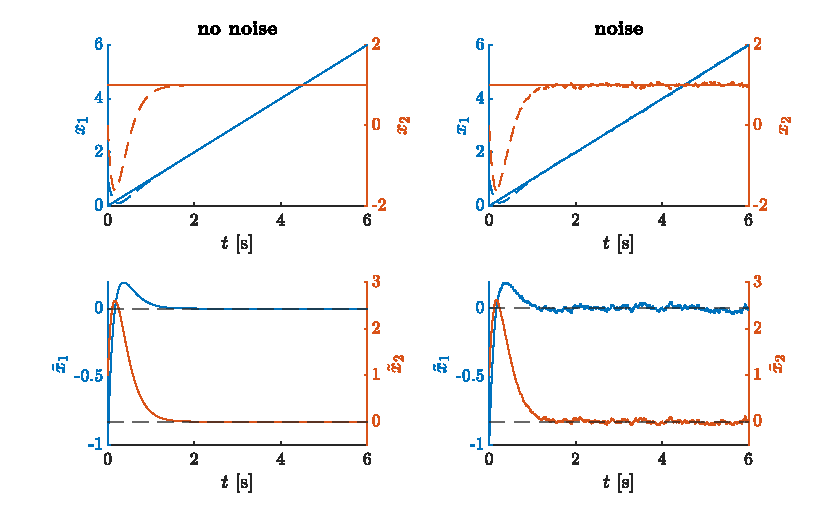
\includegraphics{figures/ex6_p1.pdf}

the blue and orange colors represent the states $x_1$ and $x_2$ respectively, the true state is shown by a solid line, and the estimated state is shown by a dashed line. 

\emph{The reduced state observer} is given as 
\begin{align*}
    \dot w &= \left(0 - l\right)\,w + \left(0 + 0 - 0 - l\,1\,l\right)\,y, & \hat x_1 &= y, \quad \hat x_2 = w + l\,y, \\
    \dot w &= -l\,w - l^2\,y, & \hat x_1 &= y, \quad \hat x_2 = w + l\,y, 
\end{align*}

The figure below gives the simulation of the full-order observer with the poles at $l = 5$\,rad/s. (placing the poles similar to the full-order observer)

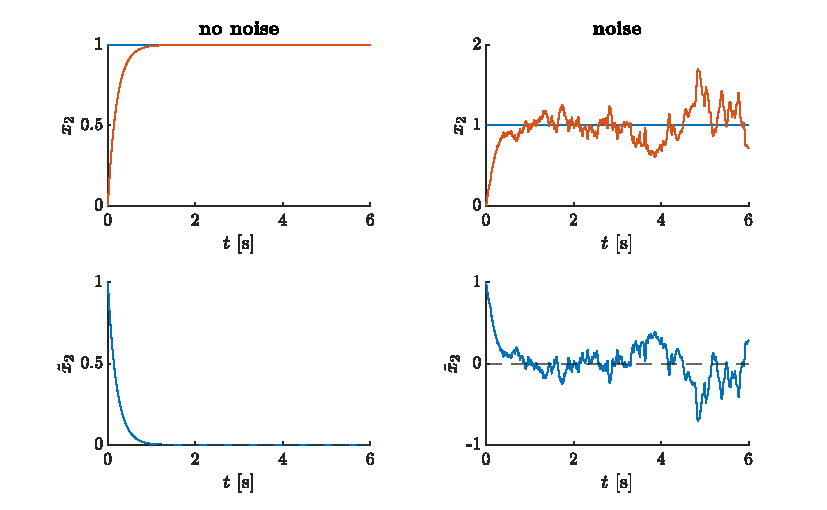
\includegraphics{figures/ex6_p2.pdf}

\fbox{
    \parbox{0.95\textwidth}{
        With the reduced order observer, the noise directly affects the observed 'state' since $x \propto y$ but in the full order observer, the noise is filtered since $\dot x \propto y$.
    }
}

\subsection*{Code}
\begin{matlabcode}
% states 
A = [0 1; 0 0];
C = [1, 0];
system = @(t,y) A*y;

% simulation 
y0 = [0; 1];
tspan = linspace(0,6,5000);
[t_true,y_true] = ode45(@(t,y) system(t,y),tspan,y0);
% adding noise
y_noise = y_true(:,1) + (rand(size(t_true)) - 0.5)*0.5;

% simulation of full-order observer
y0 = [1; 0];
y_val = @(t) interp1(t_true, y_true(:,1), t, 'spline');
[t_fo,y_fo] = ode45(@(t,y) full_order(y,y_val(t),A,C), tspan, y0);
y_temp = interp1(t_true, y_true, t_fo, 'spline');
e_fo = y_temp - y_fo;

% simulation of full-order observer with noise
y_valN = @(t) interp1(t_true, y_noise(:,1), t, 'spline');
[t_foN,y_foN] = ode45(@(t,y) full_order(y,y_valN(t),A,C), tspan, y0);
y_temp = interp1(t_true, y_true, t_foN, 'spline');
e_foN = y_temp - y_foN;

% simulation of reduced-order observer 
y0 = 0;
[t_ro,w] = ode45(@(t,y) reduced_order(y,y_val(t)),tspan,y0);
x2hat = w + 5 * y_val(t_ro);
y_temp = interp1(t_true, y_true(:,2), t_ro, 'spline');
e_ro = y_temp - x2hat;

% simulation of reduced-order observer (with noise)
[t_roN,w] = ode45(@(t,y) reduced_order(y,y_valN(t)),tspan,y0);
x2hatN = w + 5 * y_val(t_roN);
y_temp = interp1(t_true, y_true(:,2), t_roN, 'spline');
e_roN = y_temp - x2hatN;

%% functions
function xdot = full_order(x,y,A,C)
    K = [2*5; 5^2]; % feedback gain 
    xdot = A * x + K*(y - C * x);
end

function wdot = reduced_order(w,y)
    L = 5; % feedback gain 
    wdot = -L * w - L^2 * y;
end
\end{matlabcode}